\documentclass[11pt,a4paper]{article}

\usepackage[left=2cm,text={17cm,24cm},top=3cm]{geometry}
\usepackage[slovak]{babel}
\usepackage[utf8]{inputenc}
\usepackage[T1]{fontenc}

\usepackage{url}
\usepackage{enumerate}

\usepackage{tikz}
\usepackage{float}
\usepackage{xcolor}
\usepackage{siunitx}
\usepackage{comment}
\usepackage{amsmath}
\usepackage{amssymb}
\usepackage{accents}
\usepackage{listings}
\usepackage{csquotes}
\usepackage{hyperref}
\usepackage{textcomp}
\usepackage{amsfonts}
\usepackage{breakurl}
\usepackage{etoolbox}
\usepackage{graphicx}
\usepackage{multicol}
\usepackage{multirow}
\usepackage{supertabular}
\usepackage[titles]{tocloft}

\renewcommand{\cftdot}{}
\newcommand{\red}[1]{\textcolor{red}{#1}}
\newcommand{\blue}[1]{\textcolor{blue}{#1}}

\definecolor{OliveGreen}{rgb}{0,0.7,0}
\newcommand{\green}[1]{\textcolor{OliveGreen}{#1}}
\newcommand{\TODO}{\textbf{\textcolor{red}{TODO}}} % red bold TODO
\newcommand{\D}{\Delta}
\newcommand{\EOT}{\Delta^\omega} % end of tape
\newcommand{\UL}[1]{\underbar{$#1$}} % underline

\setlength\parindent{0pt}

\def\UrlBreaks{\do\/\do-}
\newcommand{\tilda}{\raisebox{0.5ex}{\texttildelow}}

\usepackage{makecell}
\renewcommand\theadalign{bc}
\renewcommand\theadfont{\bfseries}
\renewcommand\theadgape{\Gape[4pt]}
\renewcommand\cellgape{\Gape[4pt]}

\graphicspath{{.}}
\patchcmd{\thebibliography}{\section*{\refname}}{}{}{}

\begin{document}

\begin{titlepage}
    \begin{center}
        \Huge
        \textsc{
            Fakulta informačních technologií\\
            Vysoké učení technické v~Brně
        }
        \vspace{80px}
        \begin{figure}[!h]
            \centering
            
\includegraphics[scale=0.3]{img/vutbr-fit-logo.eps}
        \end{figure}
        \\[15mm]
        \Huge{
            \textbf{
                TIN
            }
        }
        \\[1.5mm]
        \huge{
            \textbf{
                Teoretická informatika
            }
        }
        \\[2.5em]
        \LARGE{
            \textbf{
                3. domáca úloha
            }
        }
        \vfill
    \end{center}
        \Large{
            Adrián Tóth (xtotha01)\hfill \today
        }
\end{titlepage}

\setlength{\parskip}{0pt}
\hypersetup{hidelinks}\tableofcontents
\setlength{\parskip}{0pt}

\newpage
\section{Príklad číslo 1}

\subsection{(a)}

Pre $f(0)$ je reťazec $x$ prázdny pre ktorý páska 4 obsahuje výslednú hodnotu $1$ t.j. $f(0)=1$.\\[-0.5em]

\begin{tabular}{r|l|l|l}
    &                    & \tiny{$R^41^4L^4$}   & \tiny{$R^1$} \\\hline
  1 & $\UL{\D} \EOT$ & $\UL{\D} \EOT$   & $\D \UL{\D} \EOT$    \\
  2 & $\UL{\D} \EOT$ & $\UL{\D} \EOT$   & $\UL{\D} \EOT$       \\
  3 & $\UL{\D} \EOT$ & $\UL{\D} \EOT$   & $\UL{\D} \EOT$       \\
  4 & $\UL{\D} \EOT$ & $\UL{\D} 1 \EOT$ & $\UL{\D} 1 \EOT$     \\
\end{tabular}

\hfill\\[-5mm]

Pre $f(1)$ je reťazec $x = 1$ pre ktorý páska 4 obsahuje výslednú hodnotu $1$ t.j. $f(1)=1$.\\[-0.5em]

\begin{tabular}{r|l|l|l|l|l|l|l|l|l}
    &                  &\tiny{$R^41^4L^4$}& \tiny{$R^1$}     & \tiny{$CP(3,2)$}  & \tiny{$L^3_\D$}   & \tiny{$CP(4,3)$}    &\tiny{$L^2_\D L^3_\D L^4_\D$}& \tiny{$CP(2,4)L^4$} & \\\hline
  1 & $\UL{\D} 1 \EOT$ & $\UL{\D} 1 \EOT$ & $\D \UL{1} \EOT$ & $\D \UL{1} \EOT$  & $\D \UL{1} \EOT$  & $\D \UL{1} \EOT$    & $\D \UL{1} \EOT$            & $\D \UL{1} \EOT$    & \\
  2 & $\UL{\D} \EOT$   & $\UL{\D} \EOT$   & $\UL{\D} \EOT$   & $\D \UL{\D} \EOT$ & $\D \UL{\D} \EOT$ & $\D \UL{\D} \EOT$   & $\UL{\D} \EOT$              & $\D \UL{\D} \EOT$   & ... \\
  3 & $\UL{\D} \EOT$   & $\UL{\D} \EOT$   & $\UL{\D} \EOT$   & $\D \UL{\D} \EOT$ & $\UL{\D} \EOT$    & $\D 1 \UL{\D} \EOT$ & $\UL{\D} 1 \EOT$            & $\UL{\D} 1 \EOT$    & \\
  4 & $\UL{\D} \EOT$   & $\UL{\D} 1 \EOT$ & $\UL{\D} 1 \EOT$ & $\UL{\D} 1 \EOT$  & $\UL{\D} 1 \EOT$  & $\D 1 \UL{\D} \EOT$ & $\UL{\D} 1 \EOT$            & $\UL{\D} 1 \EOT$    & \\
\end{tabular}

\begin{flushright}
  \begin{tabular}{r|l|l|l}
        &\tiny{$CP(3,4)$}    & \tiny{$L^2_\D L^3_\D L^4_\D$} & \tiny{$R^1$}        \\\hline
        &$\D \UL{1} \EOT$    & $\D \UL{1} \EOT$              & $\D 1 \UL{\D} \EOT$ \\
    ... &$\D \UL{\D} \EOT$   & $\UL{\D} \EOT$                & $\UL{\D} \EOT$      \\
        &$\D 1 \UL{\D} \EOT$ & $\UL{\D} 1 \EOT$              & $\UL{\D} 1 \EOT$    \\
        &$\D 1 \UL{\D} \EOT$ & $\UL{\D} 1 \EOT$              & $\UL{\D} 1 \EOT$    \\
  \end{tabular}
\end{flushright}

Pre $f(2)$ je reťazec $x = 11$ pre ktorý páska 4 obsahuje výslednú hodnotu $11$ t.j. $f(2)=2$.\\[-0.5em]

\begin{tabular}{r|l|l|l|l|l|l|l|l|l}
    &                    &\tiny{$R^41^4L^4$}  & \tiny{$R^1$}       & \tiny{$CP(3,2)$}   & \tiny{$L^3_\D$}    & \tiny{$CP(4,3)$}    &\tiny{$L^2_\D L^3_\D L^4_\D$}& \tiny{$CP(2,4)L^4$} & \\\hline
  1 & $\UL{\D} 1 1 \EOT$ & $\UL{\D} 1 1 \EOT$ & $\D \UL{1} 1 \EOT$ & $\D \UL{1} 1 \EOT$ & $\D \UL{1} 1 \EOT$ & $\D \UL{1} 1 \EOT$  & $\D \UL{1} 1 \EOT$          & $\D \UL{1} 1 \EOT$  & \\
  2 & $\UL{\D} \EOT$     & $\UL{\D} \EOT$     & $\UL{\D} \EOT$     & $\D \UL{\D} \EOT$  & $\D \UL{\D} \EOT$  & $\D \UL{\D} \EOT$   & $\UL{\D} \EOT$              & $\D \UL{\D} \EOT$   & ... \\
  3 & $\UL{\D} \EOT$     & $\UL{\D} \EOT$     & $\UL{\D} \EOT$     & $\D \UL{\D} \EOT$  & $\UL{\D} \EOT$     & $\D 1 \UL{\D} \EOT$ & $\UL{\D} 1 \EOT$            & $\UL{\D} 1 \EOT$    & \\
  4 & $\UL{\D} \EOT$     & $\UL{\D} 1 \EOT$   & $\UL{\D} 1 \EOT$   & $\UL{\D} 1 \EOT$   & $\UL{\D} 1 \EOT$   & $\D 1 \UL{\D} \EOT$ & $\UL{\D} 1 \EOT$            & $\UL{\D} 1 \EOT$    & \\
\end{tabular}

\begin{center}
  \begin{tabular}{r|l|l|l|l|l|l|l}
        &\tiny{$CP(3,4)$}    & \tiny{$L^2_\D L^3_\D L^4_\D$} & \tiny{$R^1$}       & \tiny{$CP(3,2)$}    & \tiny{$L^3_\D$}     & \tiny{$CP(4,3)$}    & \\\hline
        &$\D \UL{1} 1 \EOT$  & $\D \UL{1} 1 \EOT$            & $\D 1 \UL{1} \EOT$ & $\D 1 \UL{1} \EOT$  & $\D 1 \UL{1} \EOT$  & $\D 1 \UL{1} \EOT$  & \\
    ... &$\D \UL{\D} \EOT$   & $\UL{\D} \EOT$                & $\UL{\D} \EOT$     & $\D 1 \UL{\D} \EOT$ & $\D 1 \UL{\D} \EOT$ & $\D 1 \UL{\D} \EOT$ & ... \\
        &$\D 1 \UL{\D} \EOT$ & $\UL{\D} 1 \EOT$              & $\UL{\D} 1 \EOT$   & $\D 1 \UL{\D} \EOT$ & $\UL{\D} 1 \EOT$    & $\D 1 \UL{\D} \EOT$ & \\
        &$\D 1 \UL{\D} \EOT$ & $\UL{\D} 1 \EOT$              & $\UL{\D} 1 \EOT$   & $\UL{\D} 1 \EOT$    & $\UL{\D} 1 \EOT$    & $\D 1 \UL{\D} \EOT$ & \\
  \end{tabular}
\end{center}

\begin{flushright}
  \begin{tabular}{r|l|l|l|l|l}
        & \tiny{$L^2_\D L^3_\D L^4_\D$} & \tiny{$CP(2,4)L^4$} & \tiny{$CP(3,4)$}      & \tiny{$L^2_\D L^3_\D L^4_\D$} & \tiny{$R^1$}          \\\hline
        & $\D 1 \UL{1} \EOT$            & $\D 1 \UL{1} \EOT$  & $\D 1 \UL{1} \EOT$    & $\D 1 \UL{1} \EOT$            & $\D 1 1 \UL{\D} \EOT$ \\
    ... & $\UL{\D} 1 \EOT$              & $\D 1 \UL{\D} \EOT$ & $\D 1 \UL{\D} \EOT$   & $\UL{\D} 1 \EOT$              & $\UL{\D} 1 \EOT$      \\
        & $\UL{\D} 1 \EOT$              & $\UL{\D} 1 \EOT$    & $\D 1 \UL{\D} \EOT$   & $\UL{\D} 1 \EOT$              & $\UL{\D} 1 \EOT$      \\
        & $\UL{\D} 1 \EOT$              & $\D \UL{1} \EOT$    & $\D 1 1 \UL{\D} \EOT$ & $\UL{\D} 1 1 \EOT$            & $\UL{\D} 1 1 \EOT$    \\
  \end{tabular}
\end{flushright}

Hodnoty na páske číslo $4$ $TS$ $M$ pre jednotlivé $x$ sú uvedené dole v tabuľke.

\begin{center}
\begin{tabular}{l|l|l|l}
  \multicolumn{1}{c|}{\thead{$x$}} & \multicolumn{1}{c|}{\thead{unárny\\zápis $x$}} & \multicolumn{1}{c|}{\thead{obsah pásky č. $4$\\po zastavení $TS$ $M$}} & \multicolumn{1}{c}{\thead{hodnota čísla\\na páske č. $4$}} \\
  \hline
  $0$ & $\varepsilon$ & $\UL{\D} 1 \EOT$        & $1$ \\
  $1$ & $1$           & $\UL{\D} 1 \EOT$        & $1$ \\
  $2$ & $11$          & $\UL{\D} 11 \EOT$       & $2$ \\
  $3$ & $111$         & $\UL{\D} 111 \EOT$      & $3$ \\
  $4$ & $1111$        & $\UL{\D} 11111 \EOT$    & $5$ \\
  $5$ & $11111$       & $\UL{\D} 11111111 \EOT$ & $8$ \\
\end{tabular}
\end{center}

Pre $f(0),f(1),f(2),f(3),f(4),f(5)$ odpovedá rada čísel $1,1,2,3,5,8$. Na základe získaných hodnôt ktoré sú uvedné vyššie v tabuľke a faktu, že sa jedná o veľmi známu radu čísel vyplýva, že funkcia~$f$ generuje čísla z Fibonacciho rady.

\subsection{(b)}

Funkciu $f$ môžeme definovať ako parciálne rekurzívnu funckiu nasledujúcim spôsobom

\begin{center}
\begin{tabular}{rcl}
  $f(x)$   & \hspace{-3mm}$=$\hspace{-3mm} & $\pi_1^2 \circ h(x)$\\
  $h(x+1)$ & \hspace{-3mm}$=$\hspace{-3mm}      & $(\pi_2^2 \circ h(x), plus(\pi_1^2 \circ h(x),\pi_2^2 \circ h(x)))$\\
  $h(0)$   & \hspace{-3mm}$=$\hspace{-3mm}      & $(1,1)$
\end{tabular}
\end{center}

Demonštrácia na príklade pre $f(5)$

\begin{center}
\begin{tabular}{rcl}
$f(5)$ & \hspace{-3mm}$=$\hspace{-3mm} & $\pi_1^2 \circ h(5)$\\
       & \hspace{-3mm}$=$\hspace{-3mm} & $\pi_1^2 (8,13)$\\
       & \hspace{-3mm}$=$\hspace{-3mm} & $8$\\
\\[-0.9em]
\hline\\[-0.75em]
$h(5)$ & \hspace{-3mm}$=$\hspace{-3mm} & $(\pi_2^2 \circ h(4), plus(\pi_1^2 \circ h(4),\pi_2^2 \circ h(4)))$\\
       & \hspace{-3mm}$=$\hspace{-3mm} & $(\pi_2^2 (5, 8), plus(\pi_1^2 (5, 8),\pi_2^2 (5, 8)))$\\
       & \hspace{-3mm}$=$\hspace{-3mm} & $(8, plus(5,8))$\\
       & \hspace{-3mm}$=$\hspace{-3mm} & $(8,13)$\\
\\[-0.9em]
\hline\\[-0.75em]
$h(4)$ & \hspace{-3mm}$=$\hspace{-3mm} & $(\pi_2^2 \circ h(3), plus(\pi_1^2 \circ h(3),\pi_2^2 \circ h(3)))$\\
       & \hspace{-3mm}$=$\hspace{-3mm} & $(\pi_2^2 (3, 5), plus(\pi_1^2 (3, 5),\pi_2^2 (3, 5)))$\\
       & \hspace{-3mm}$=$\hspace{-3mm} & $(5, plus(3,5))$\\
       & \hspace{-3mm}$=$\hspace{-3mm} & $(5,8)$\\
\\[-0.9em]
\hline\\[-0.75em]
$h(3)$ & \hspace{-3mm}$=$\hspace{-3mm} & $(\pi_2^2 \circ h(2), plus(\pi_1^2 \circ h(2),\pi_2^2 \circ h(2)))$\\
       & \hspace{-3mm}$=$\hspace{-3mm} & $(\pi_2^2 (2, 3), plus(\pi_1^2 (2, 3),\pi_2^2 (2, 3)))$\\
       & \hspace{-3mm}$=$\hspace{-3mm} & $(3, plus(2,3))$\\
       & \hspace{-3mm}$=$\hspace{-3mm} & $(3,5)$\\
\\[-0.9em]
\hline\\[-0.75em]
$h(2)$ & \hspace{-3mm}$=$\hspace{-3mm} & $(\pi_2^2 \circ h(1), plus(\pi_1^2 \circ h(1),\pi_2^2 \circ h(1)))$\\
       & \hspace{-3mm}$=$\hspace{-3mm} & $(\pi_2^2 (1, 2), plus(\pi_1^2 (1, 2),\pi_2^2 (1, 2)))$\\
       & \hspace{-3mm}$=$\hspace{-3mm} & $(2, plus(1,2))$\\
       & \hspace{-3mm}$=$\hspace{-3mm} & $(2,3)$\\
\\[-0.9em]
\hline\\[-0.75em]
$h(1)$ & \hspace{-3mm}$=$\hspace{-3mm} & $(\pi_2^2 \circ h(0), plus(\pi_1^2 \circ h(0),\pi_2^2 \circ h(0)))$\\
       & \hspace{-3mm}$=$\hspace{-3mm} & $(\pi_2^2 (1, 1), plus(\pi_1^2 (1, 1),\pi_2^2 (1, 1)))$\\
       & \hspace{-3mm}$=$\hspace{-3mm} & $(1, plus(1,1))$\\
       & \hspace{-3mm}$=$\hspace{-3mm} & $(1,2)$\\
\\[-0.9em]
\hline\\[-0.75em]
$h(0)$ & \hspace{-3mm}$=$\hspace{-3mm} & $(1, 1)$\\
\end{tabular}
\end{center}

\newpage
\section{Príklad číslo 2}

Nevypracované.

\newpage
\section{Príklad číslo 3}

Dôkaz:\\[-0.5em]

\hspace{5mm}1.) Dôkaz sporom pre '$\subseteq$'

\begin{flushright}
\begin{minipage}{0.92\textwidth}
  Predpokladajme, že platí
  \begin{center}
    $\mathcal{O}(3^{2n}) \subseteq \mathcal{O}(2^{3n})$
  \end{center}
  Potom
  \begin{center}
    $\exists c \in \mathbb{R}^{+} \ \exists n_{0} \in \mathbb{N} \ \forall n \geq n_{0}: 3^{2n} \leq c\hspace{0.5mm}2^{3n}$
  \end{center}
  Môžeme krátiť vzhľadom ku tomu, že $3^{2n} \neq 0$ pre žiadne $n$
  \begin{center}
    $\exists c \in \mathbb{R}^{+} \ \exists n_{0} \in \mathbb{N} \ \forall n \geq n_{0}: \frac{c2^{3n}}{3^{2n}} \geq 1$
  \end{center}
  Uvážme\\[-3.5em]
  \begin{center}
    $$\lim_{n\to\infty} \frac{c2^{3n}}{3^{2n}}$$
  \end{center}
  Vypočítame hore uvedenú limitu\\[-3.5em]
  \begin{center}
    $$\lim_{n\to\infty} \frac{c2^{3n}}{3^{2n}} = \lim_{n\to\infty} \frac{c\left(2^3\right)^n}{\left(3^2\right)^n} = \lim_{n\to\infty} \frac{c\hspace{0.2mm}8^n}{9^n} = \lim_{n\to\infty} c\frac{8^n}{9^n} = \lim_{n\to\infty} c{\left({\frac{8}{9}}\right)}^n = c\hspace{0.2mm}0 = 0$$
  \end{center}
  Nemôže súčastne platiť, že\\[-3.5em]
  \begin{center}
    $$\lim_{n\to\infty} \frac{c2^{3n}}{3^{2n}} = 0$$
  \end{center}
  a
  \begin{center}
    $\exists c \in \mathbb{R}^{+} \ \exists n_{0} \in \mathbb{N} \ \forall n \geq n_{0}: \frac{c2^{3n}}{3^{2n}} \geq 1$
  \end{center}
  z čoho vyplýva, že sa jedná o spor z čoho vyplýva, že
  \begin{center}
    $\mathcal{O}(3^{2n}) \nsubseteq \mathcal{O}(2^{3n})$
  \end{center}
\end{minipage}
\end{flushright}

\hspace{5mm}2.) Dôkaz sporom pre '$\supseteq$'

\begin{flushright}
\begin{minipage}{0.92\textwidth}
  Predpokladajme, že platí
  \begin{center}
    $\mathcal{O}(3^{2n}) \supseteq \mathcal{O}(2^{3n})$
  \end{center}
  Potom
  \begin{center}
    $\exists c \in \mathbb{R}^{+} \ \exists n_{0} \in \mathbb{N} \ \forall n \geq n_{0}: c\hspace{0.5mm}3^{2n} \geq 2^{3n}$
  \end{center}
  Môžeme krátiť vzhľadom ku tomu, že $2^{3n} \neq 0$ pre žiadne $n$
  \begin{center}
    $\exists c \in \mathbb{R}^{+} \ \exists n_{0} \in \mathbb{N} \ \forall n \geq n_{0}: \frac{c3^{2n}}{2^{3n}} \geq 1$
  \end{center}
  Uvážme\\[-3.5em]
  \begin{center}
    $$\lim_{n\to\infty} \frac{c3^{2n}}{2^{3n}}$$
  \end{center}
\end{minipage}
\end{flushright}

\begin{flushright}
\begin{minipage}{0.92\textwidth}
  Vypočítame hore uvedenú limitu\\[-3.5em]
  \begin{center}
    $$\lim_{n\to\infty} \frac{c\hspace{0.2mm}3^{2n}}{2^{3n}} = \lim_{n\to\infty} \frac{c\left(3^2\right)^n}{\left(2^3\right)^n} = \lim_{n\to\infty} \frac{c\hspace{0.2mm}9^n}{8^n} = \lim_{n\to\infty} c\frac{9^n}{8^n} = \lim_{n\to\infty} c{\left({\frac{9}{8}}\right)}^n = c(+\infty) = +\infty$$
  \end{center}
  Keďže platí, že\\[-3.5em]
  \begin{center}
    $$\lim_{n\to\infty} \frac{c3^{2n}}{2^{3n}} = +\infty$$
  \end{center}
  a
  \begin{center}
    $\exists c \in \mathbb{R}^{+} \ \exists n_{0} \in \mathbb{N} \ \forall n \geq n_{0}: \frac{c3^{2n}}{2^{3n}} \geq 1$
  \end{center}
  tak z toho vyplýva, že predpokladaný vzťah platí
  \begin{center}
    $\mathcal{O}(3^{2n}) \supseteq \mathcal{O}(2^{3n})$
  \end{center}
\end{minipage}
\end{flushright}

\hspace{5mm}3.) Priamy dôkaz pre '$=$'

\begin{flushright}
\begin{minipage}{0.92\textwidth}
  Keďže z hore uvedených dôkazov platí, že
  \begin{center}
    $\mathcal{O}(3^{2n}) \nsubseteq \mathcal{O}(2^{3n})$
  \end{center}
  a
  \begin{center}
    $\mathcal{O}(3^{2n}) \supseteq \mathcal{O}(2^{3n})$
  \end{center}
  tak z toho vyplýva, že nasledujúci vzťah neplatí
  \begin{center}
    $\mathcal{O}(3^{2n}) = \mathcal{O}(2^{3n})$
  \end{center}
  teda musí platiť, že
  \begin{center}
    $\mathcal{O}(3^{2n}) \neq \mathcal{O}(2^{3n})$
  \end{center}
\end{minipage}
\end{flushright}

\newpage
\section{Príklad číslo 4}

Nevypracované.

\newpage
\section{Príklad číslo 5}

Na obrázku \ref{fig:pn} je nakreslená petriho sieť ktorá akceptuje jazyk

\begin{center}
$L = \{a^i(b^j)c^k \in \{a,b,c,(,)\}^* \ | \ i \geq j = k\}$
\end{center}

\hfill\\[-4em]

\begin{figure}[H]
  \centering
  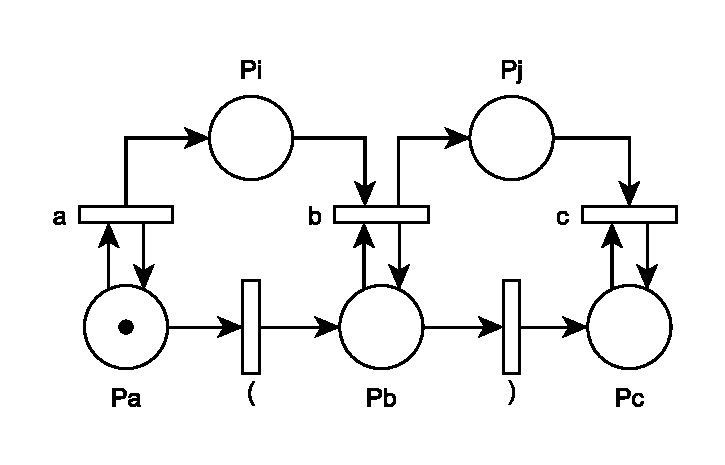
\includegraphics[scale=1.1]{img/pn.eps}
  \caption{Petriho sieť.}
  \label{fig:pn}
\end{figure}

\phantom{\cite{TIN}} % hiddes text but creates a line according to the text size

\newpage
\section{Literatúra}
\bibliographystyle{slovakiso}
\begin{flushleft}
    \bibliography{quotation}
\end{flushleft}

\end{document}
